\documentclass[final]{beamer}
% http://tex.stackexchange.com/questions/56205/wrapfigure-beamer-style
\usepackage{color}
\usepackage{transparent}
%\usepackage{enumitem}
%\usepackage{cutwin}
%\usetheme{RJH}
\usetheme{irishep}
%\usetheme{Bergen}
\usepackage[orientation=portrait,size=a0,scale=1.4,debug]{beamerposter}
\usepackage[absolute,overlay]{textpos}
\setlength{\TPHorizModule}{1cm}
\setlength{\TPVertModule}{1cm}
\beamertemplatenavigationsymbolsempty
% RGB (145,201,219), #91C9DB
%\definecolor{mybluelabel}{RGB}{145,201,219}
% RGB (48,174,228), #30AEE4
\definecolor{mybluelabel}{RGB}{48,174,228}

% Turn off list indentation
%\setlist[itemize]{leftmargin=*}

\begin{document}
\begin{frame}{} 

\begin{textblock}{80.0}(2,2)
\begin{center}
%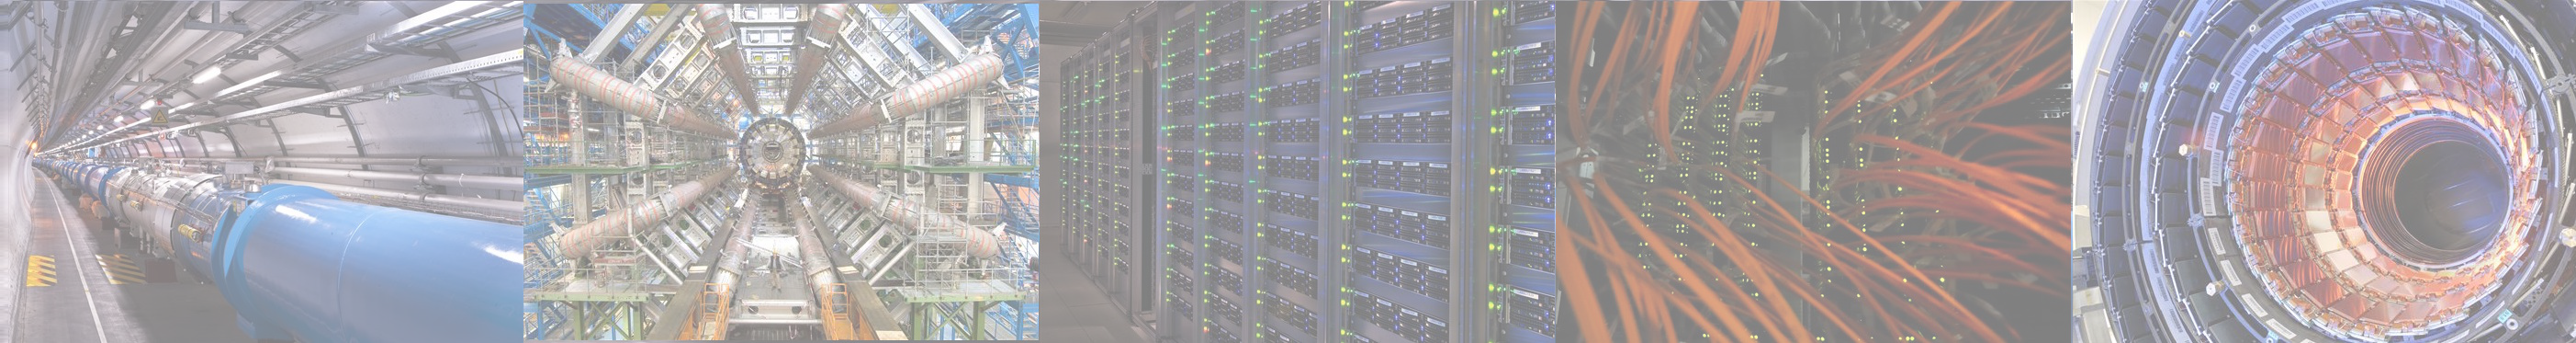
\includegraphics[width=1.00\textwidth]{images/s2i2-banner-50percent.png}
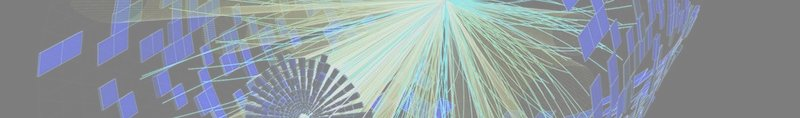
\includegraphics[width=1.00\textwidth]{images/Tprime-200pu-PhaseII-black-arctic-main-image-slice.jpg}
\end{center}
\end{textblock}

\begin{textblock}{84.0}(0,3)
\begin{center}
\begin{Huge}
%\color{white}{
\textbf{
Institute for Research and Innovation in Software \\ 
~~for High Energy Physics (IRIS-HEP)
}
%}
\end{Huge}
\end{center}
\end{textblock}

\begin{textblock}{84.0}(2,8.8)
\begin{center}
\begin{Large}
\textbf{
PIs: Peter Elmer (Princeton Univ.), Gordon Watts (Univ. of Washington)\\ 
, Brian Bockelman (Morgridge Institute)
}
\end{Large}
\end{center}
\end{textblock}


\begin{textblock}{80.0}(2,14)
\begin{block}{Science Driver: Discoveries beyond the Standard Model of Particle Physics}

\begin{textblock}{16.0}(2,16)
\begin{figure}[H]
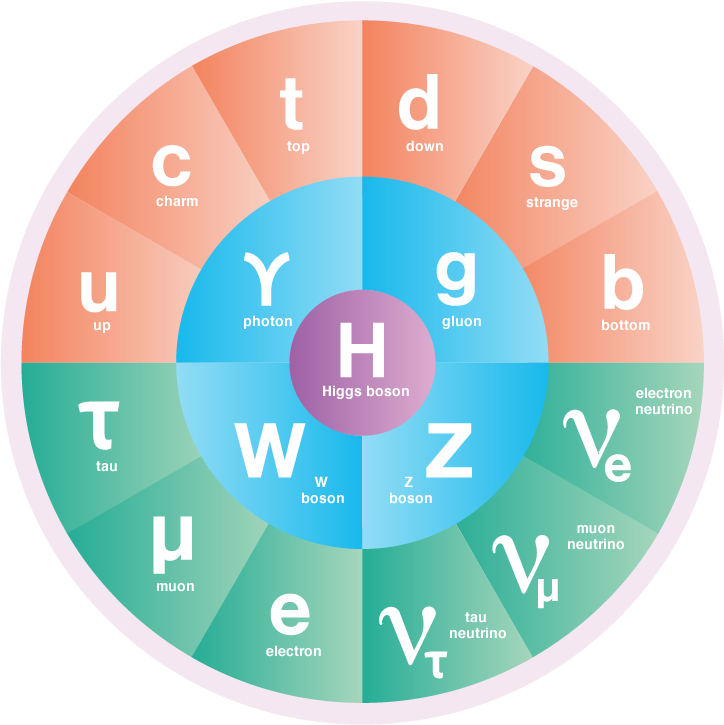
\includegraphics[width=0.87\textwidth]{images/standard_model_ai.png}
\end{figure}
\end{textblock}

\begin{textblock}{50.0}(20,18)
{\it From ``Building for Discovery - Strategic Plan for U.S. Particle Physics in the Global \\
Context'' - Report of the Particle Physics Project Prioritization Panel (P5):}

\begin{center}
\begin{enumerate}
\item Use the Higgs boson as a new tool for discovery
\item Pursue the physics associated with neutrino mass
\item Identify the new physics of dark matter
\item Understand cosmic acceleration: dark matter and inflation
\item Explore the unknown: new particles, interactions, and physical principles
\end{enumerate}
\end{center}
\end{textblock}

\begin{textblock}{16.0}(64,16)
\begin{figure}[H]
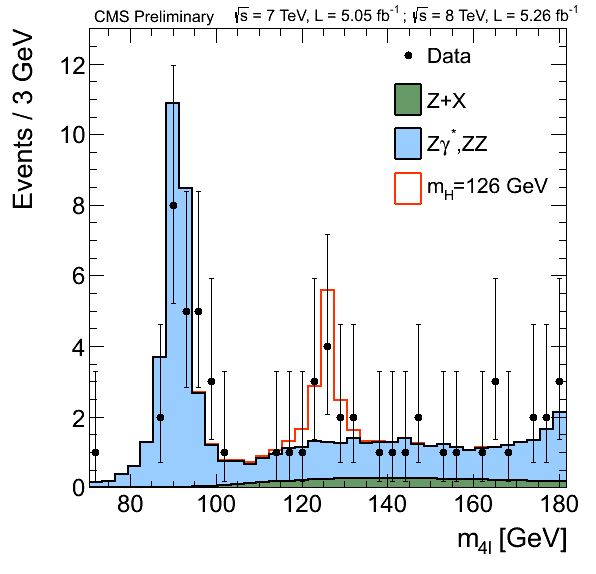
\includegraphics[width=0.95\textwidth]{images/Fig4-ZZMass_7Plus8TeV_70-180_3GeV.png}
\end{figure}
\end{textblock}

\end{block}
\end{textblock}

%%%%%%%%%%%%%%%%%%%%%%%%%%%%%%%%%%%%%%%%%%%%%%%%%%%%%%%%%%%%%%%%%%%%%%%%%%%%%%


\begin{textblock}{20.0}(2,32)
\begin{block}{The IRIS-HEP Software Institute}
\begin{textblock}{20.0}(2,34)
IRIS-HEP aims to develop the state of the art software cyberinfrastructure required for the challenges of data intensive scientific research at the High Luminosity Large Hadron Collider (HL-LHC) at CERN, and other planned HEP experiments of the 2020’s. These facilities are discovery machines which aim to understand the fundamental building blocks of nature and their interactions.
\end{textblock}
\end{block}
\end{textblock}


\begin{textblock}{32.0}(22,30)
\begin{figure}[tbph]
\centering
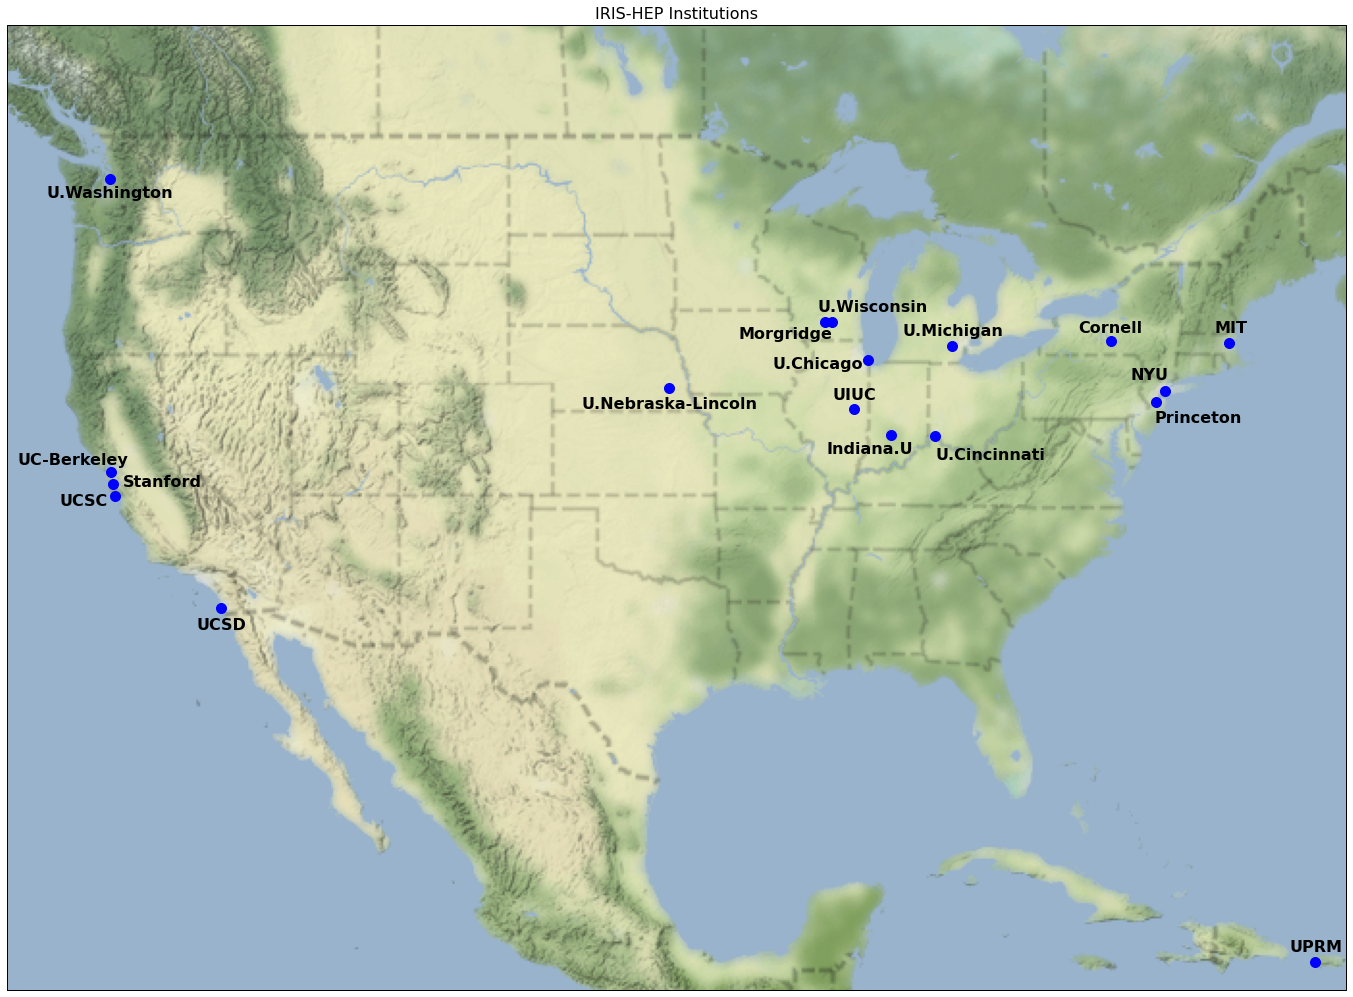
\includegraphics[width=0.90\textwidth]{images/iris-hep-map-V1.png}
\end{figure}
%\end{block}
\end{textblock}

\begin{textblock}{28.0}(54,32)
\begin{block}{An Intellectual Hub for the HEP Community}
\begin{textblock}{26.0}(54,34)
\begin{figure}[tbph]
\centering
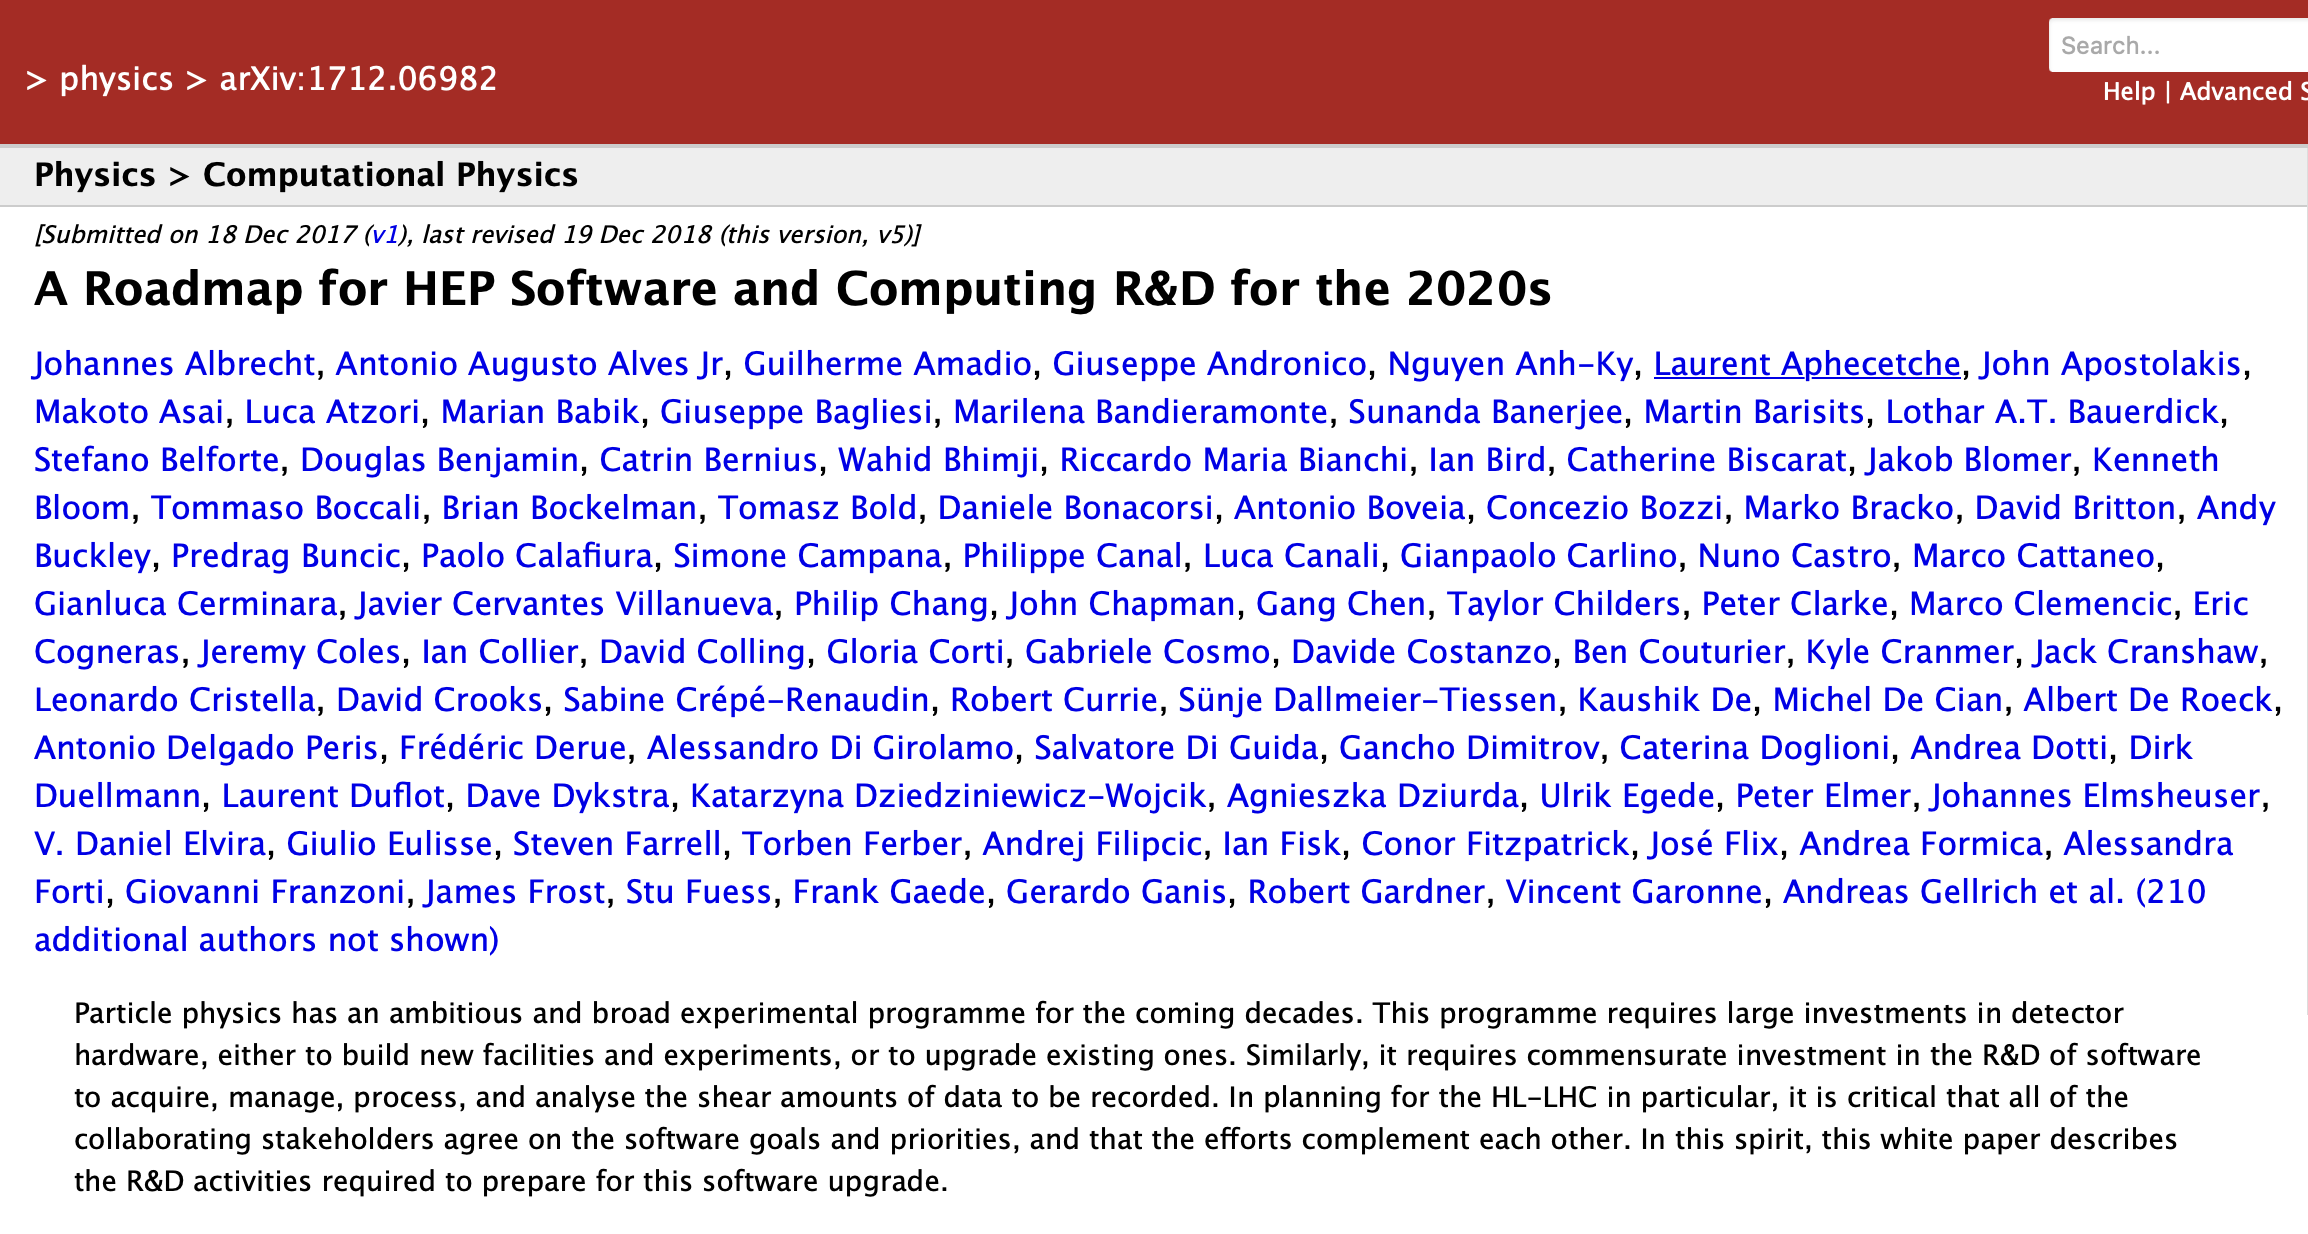
\includegraphics[width=1.07\textwidth]{images/20230925-arxiv-roadmap.png}
\end{figure}
\end{textblock}
\end{block}
\end{textblock}




%%%%%%%%%%%%%%%%%%%%%%%%%%%%%%%%%%%%%%%%%%%%%%%%%%%%%%%%%%%%%%%%%%%%%%%%%%%%%%
\begin{textblock}{25.0}(2,52)
\begin{block}{A Python Data Science Ecosystem}
\begin{textblock}{25.0}(2,54)
\begin{figure}[tbph]
\centering
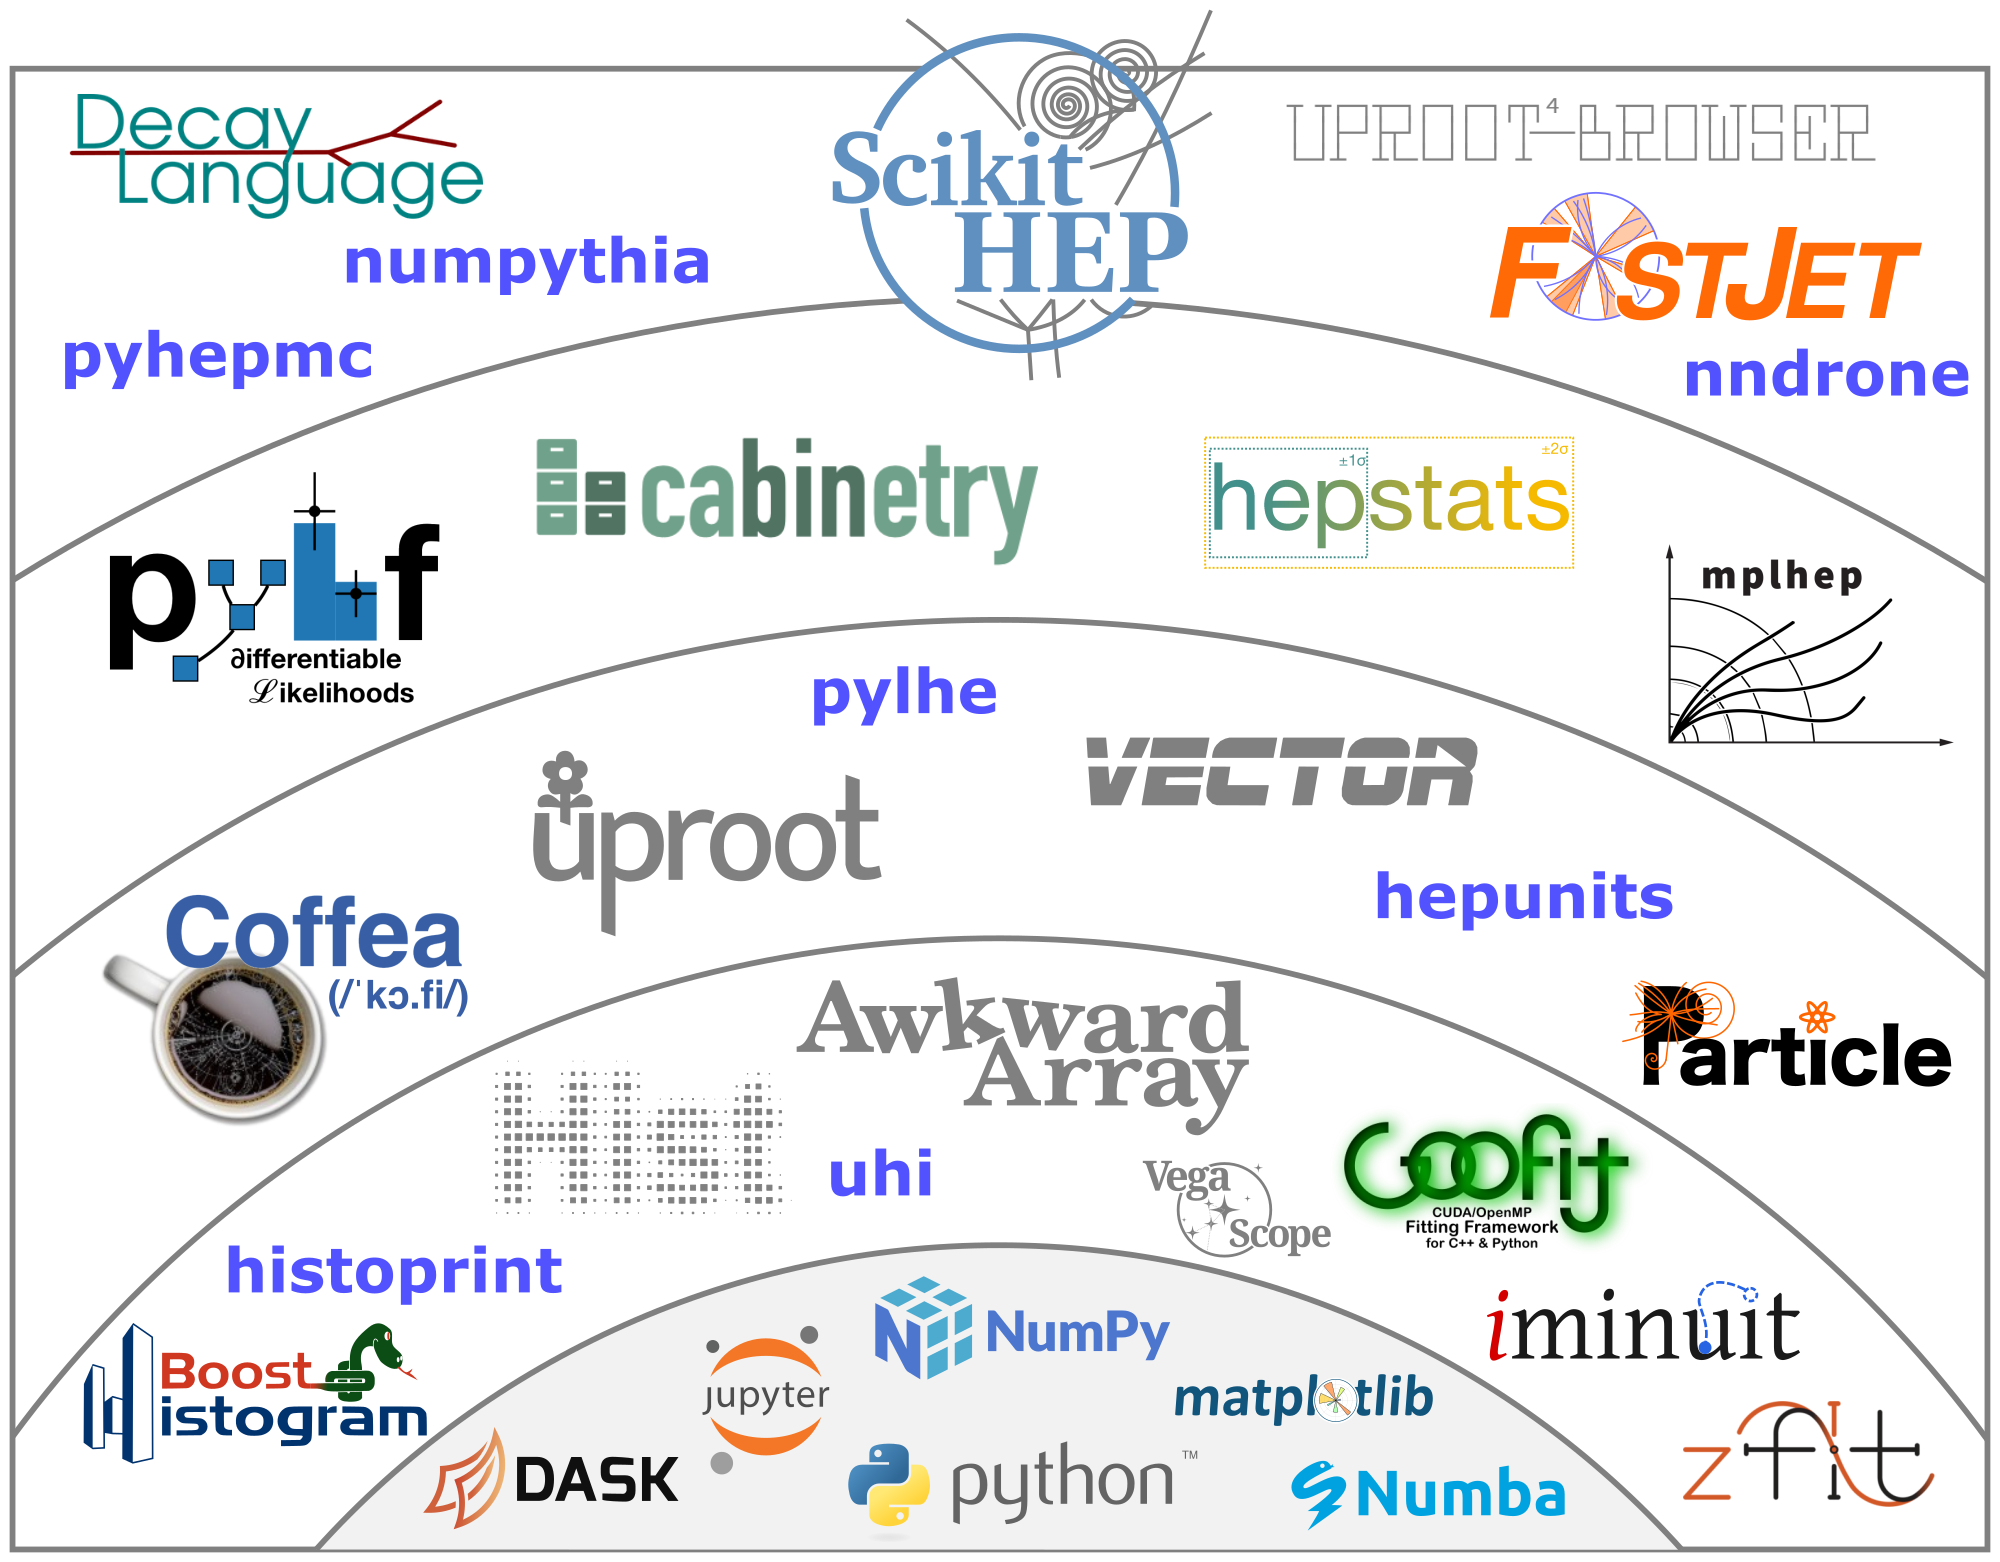
\includegraphics[width=1.00\textwidth]{images/scikit-hep-shells-hep.png}
\end{figure}
We develop sustainable analysis tools to extend the physics reach of the HL-LHC experiments by creating greater functionality, reducing time to insight, lowering the barriers for smaller teams, and streamlining analysis preservation, reproducibility, and reuse.
\end{textblock}
\end{block}
\end{textblock}
%%%%%%%%%%%%%%%%%%%%%%%%%%%%%%%%%%%%%%%%%%%%%%%%%%%%%%%%%%%%%%%%%%%%%%%%%%%%%%
\begin{textblock}{25.0}(29,52)
\begin{block}{Innovative Algorithms}
\begin{textblock}{25.0}(29,54)
\begin{figure}[tbph]
\centering
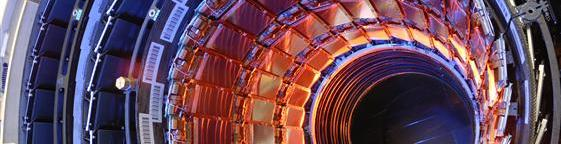
\includegraphics[width=0.90\textwidth]{images/0610026_01-A5-at-72-dpi-slice.jpg}
\end{figure}
High performant software algorithms to perform the real-time processing in the trigger and the reconstruction of both real and simulated detector data are critical components of HEP’s computing challenge, for example for charged particle tracking. 
\begin{figure}[tbph]
\centering
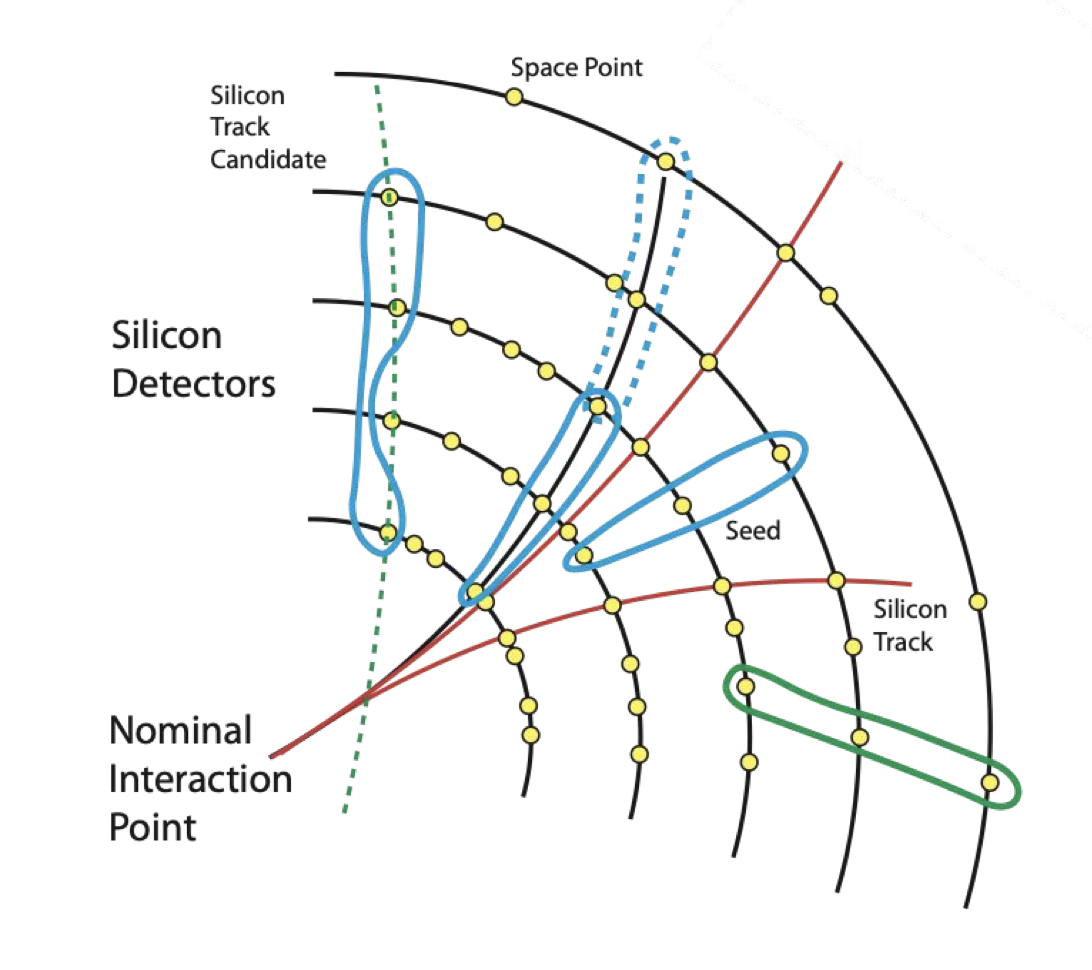
\includegraphics[width=0.90\textwidth]{images/trackreco-graphic.png}
\end{figure}
\end{textblock}
\end{block}
\end{textblock}
%%%%%%%%%%%%%%%%%%%%%%%%%%%%%%%%%%%%%%%%%%%%%%%%%%%%%%%%%%%%%%%%%%%%%%%%%%%%%%
\begin{textblock}{25.0}(56,52)
\begin{block}{Data Organization, Management, Access (DOMA)}
\begin{textblock}{25.0}(56,54)
\begin{figure}[tbph]
\centering
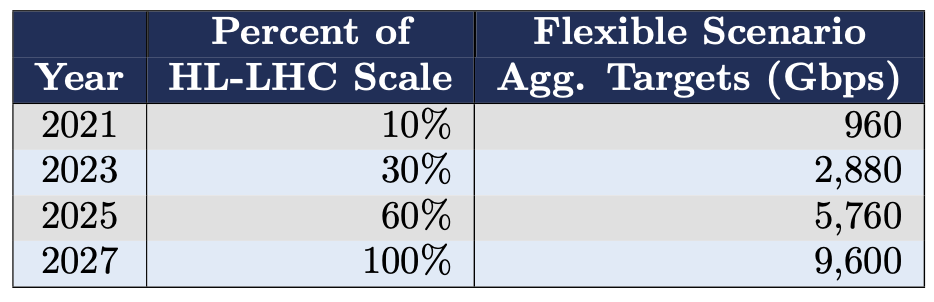
\includegraphics[width=0.90\textwidth]{images/doma-scale-challenges.png}
\end{figure}
Our DOMA program of work centers on the management and delivery of exabyte-scale production datasets and delivery of data to analysis facilities. Biennial data challenges are used to show readiness of technologies and scale.
\end{textblock}
\end{block}
\end{textblock}
%%%%%%%%%%%%%%%%%%%%%%%%%%%%%%%%%%%%%%%%%%%%%%%%%%%%%%%%%%%%%%%%%%%%%%%%%%%%%%
\begin{textblock}{25.0}(2,84)
\begin{block}{Scalable Systems Laboratory (SSL)}
\begin{textblock}{25.0}(2,86)
\begin{figure}[tbph]
\centering
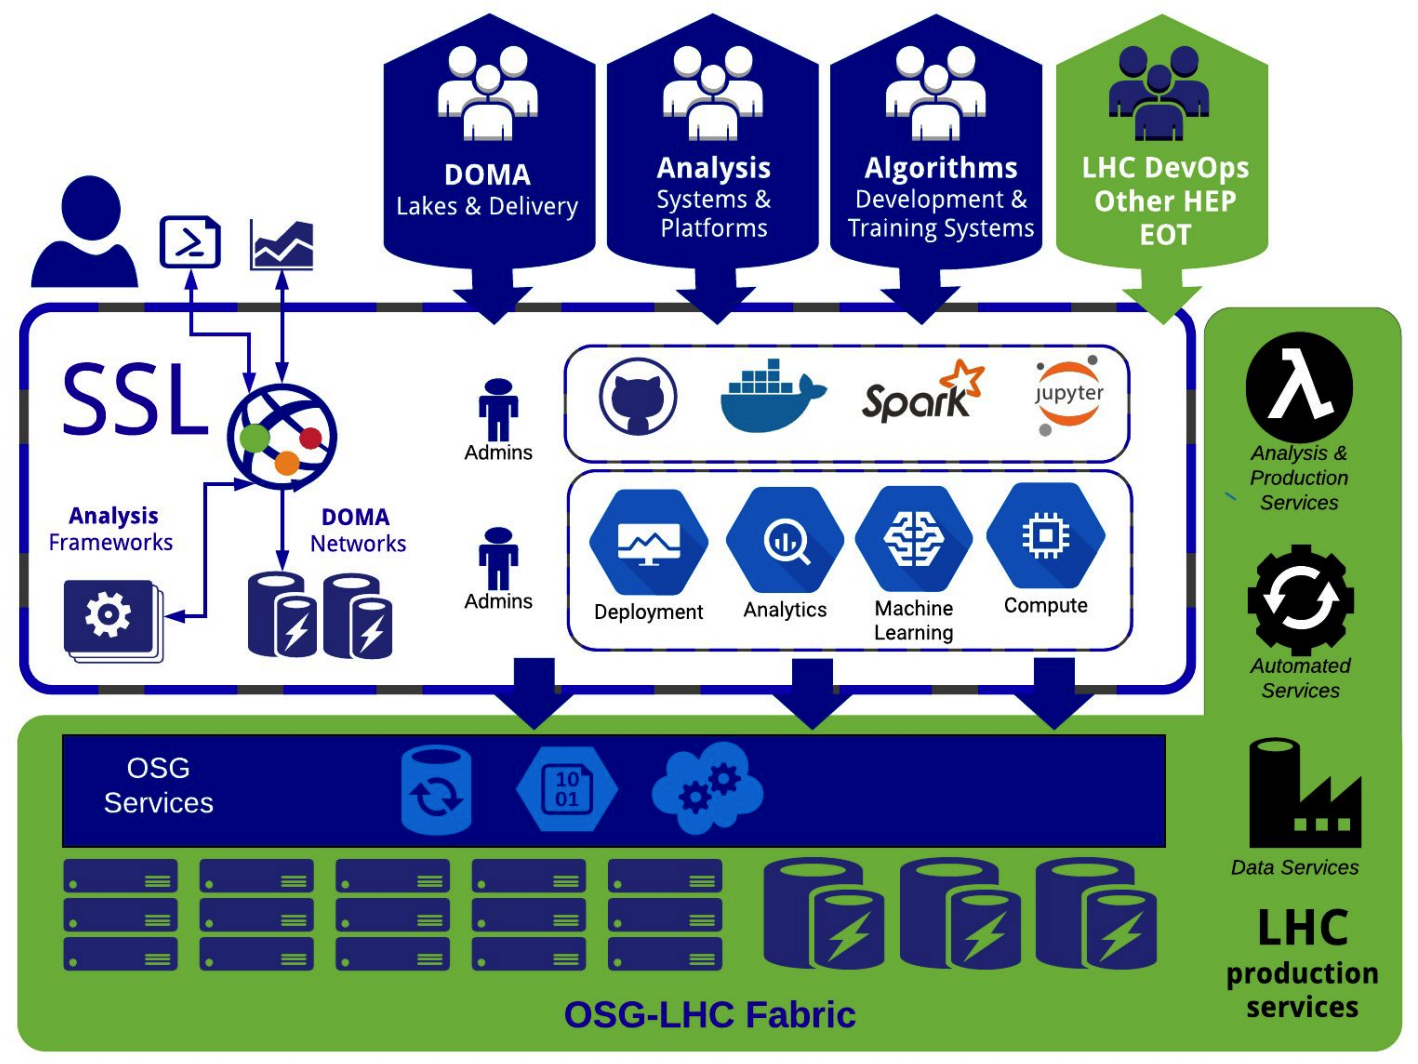
\includegraphics[width=0.75\textwidth]{images/ssl.png}
\end{figure}
The SSL provides HEP software developers with a means to transition their R\&D from conceptual toys to testbeds to production-scale prototypes as well as performs foundational systems R\&D.
\end{textblock}
\end{block}
\end{textblock}
%%%%%%%%%%%%%%%%%%%%%%%%%%%%%%%%%%%%%%%%%%%%%%%%%%%%%%%%%%%%%%%%%%%%%%%%%%%%%%
\begin{textblock}{25.0}(29,89)
\begin{block}{Distributed High Throughput Computing}
\begin{textblock}{25.0}(29,91)
\begin{figure}[tbph]
\centering

\includegraphics[width=0.75\textwidth]{images/osg-logo.png}
\end{figure}
OSG-LHC contributes to the larger mission of the OSG Consortium by evolving the production infrastructure that the LHC collaborations depend on in the USA for the HL-LHC science program. 
\end{textblock}
\end{block}
\end{textblock}
%%%%%%%%%%%%%%%%%%%%%%%%%%%%%%%%%%%%%%%%%%%%%%%%%%%%%%%%%%%%%%%%%%%%%%%%%%%%%%
\begin{textblock}{25.0}(56,70)
\begin{block}{Education, Training and Outreach}
\begin{textblock}{25.0}(56,72)
\begin{figure}[tbph]
\centering
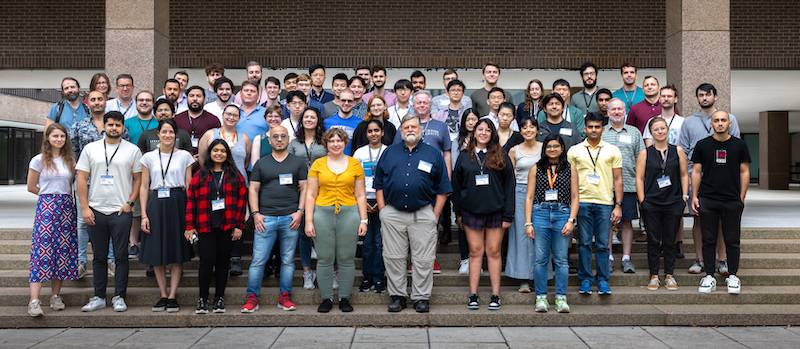
\includegraphics[width=1.00\textwidth]{images/codas-hep-2023-group-photo-thumbnail.jpg}
\end{figure}
The long term sustainability of our software efforts and science depends on a pipeline of software enabled scientists and engineers. We have implemented a scalable community basic software training program in collaboration with the HEP Software Foundation and FIRST-HEP (OAC-1829707, OAC-1829729). A large summer student program has trained more than 100 students and the annual Computational and Data Science for HEP (CoDaS-HEP) summer school provides more advanced training. A separate outreach program in partnership with QuarkNet aims to developing coding skills in high school teachers and students.
\end{textblock}
\end{block}
\end{textblock}
%%%%%%%%%%%%%%%%%%%%%%%%%%%%%%%%%%%%%%%%%%%%%%%%%%%%%%%%%%%%%%%%%%%%%%%%%%%%%%


\begin{textblock}{8.0}(4,107)
\begin{figure}[tbph]
\centering

\includegraphics[width=0.95\textwidth]{images/nsf1.jpg}
\end{figure}
\end{textblock}

\begin{textblock}{58.0}(12,108)
%\begin{block}{This poster online with links}
\begin{center}
This project is supported by National Science Foundation under Cooperative Agreements OAC-1836650 and PHY-2323298. Any opinions, findings, conclusions or recommendations expressed in this material are those of the authors and do not necessarily reflect the views of the National Science Foundation.
%\end{block}
\end{center}
\begin{center}
\Large
\url{https://iris-hep.org}
\end{center}

\end{textblock}

\begin{textblock}{8.0}(70,108)
%\begin{block}{This poster online with links}
\begin{figure}[tbph]
\centering

\includegraphics[width=1.4\textwidth]{images/Iris-hep-4-no-long-name.png}
\end{figure}
%\end{block}
\end{textblock}


\end{frame}
\end{document}
